% SkyPass architecture diagram (colour). Built by experiments/diagrams/build_diagrams.py.
% Palette: Okabe-Ito, the same colour-blind-safe set the result charts use.
\documentclass[border=4pt]{standalone}
\usepackage{tikz}
\usetikzlibrary{arrows.meta, positioning, calc, fit, backgrounds}
\definecolor{orbit}{HTML}{0072B2}
\definecolor{weather}{HTML}{009E73}
\definecolor{score}{HTML}{CC79A7}
\definecolor{plan}{HTML}{E69F00}
\definecolor{outc}{HTML}{D55E00}
\definecolor{src}{HTML}{666666}
\begin{document}
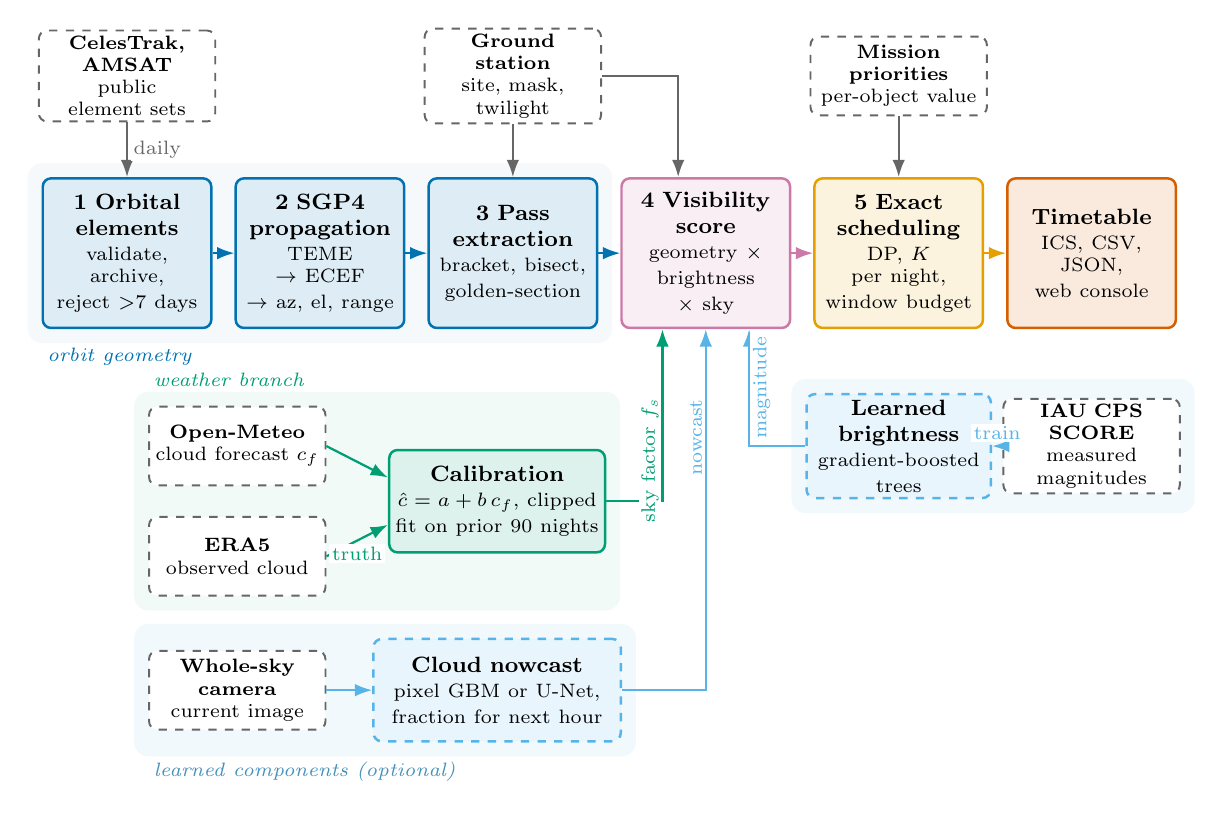
\begin{tikzpicture}[
  font=\footnotesize,
  every node/.append style={execute at begin node={\hyphenpenalty=10000\exhyphenpenalty=10000}},
  stage/.style={draw=#1, line width=0.9pt, fill=#1!13, rounded corners=3pt,
                align=center, text width=20mm, minimum height=19mm, inner sep=2pt},
  source/.style={draw=src, dashed, line width=0.7pt, fill=white, rounded corners=3pt,
                 align=center, text width=21mm, minimum height=10mm, inner sep=2pt,
                 font=\scriptsize},
  arr/.style={-{Latex[length=2.2mm, width=1.6mm]}, line width=0.8pt, draw=#1},
  lab/.style={font=\scriptsize, text=#1, inner sep=1pt, fill=white},
]
% ---------------------------------------------------------------- main row
\node[stage=orbit]   (s1) at (0,0)    {\textbf{1 Orbital}\\\textbf{elements}\\[1pt]{\scriptsize validate, archive,\\reject $>$7 days}};
\node[stage=orbit]   (s2) at (2.45,0) {\textbf{2 SGP4}\\\textbf{propagation}\\[1pt]{\scriptsize TEME $\to$ ECEF\\$\to$ az, el, range}};
\node[stage=orbit]   (s3) at (4.9,0)  {\textbf{3 Pass}\\\textbf{extraction}\\[1pt]{\scriptsize bracket, bisect,\\golden-section}};
\node[stage=score]   (s4) at (7.35,0) {\textbf{4 Visibility}\\\textbf{score}\\[1pt]{\scriptsize geometry $\times$\\brightness $\times$ sky}};
\node[stage=plan]    (s5) at (9.8,0)  {\textbf{5 Exact}\\\textbf{scheduling}\\[1pt]{\scriptsize DP, $K$ per night,\\window budget}};
\node[stage=outc]    (tt) at (12.25,0){\textbf{Timetable}\\[1pt]{\scriptsize ICS, CSV, JSON,\\web console}};
\foreach \a/\b/\c in {s1/s2/orbit, s2/s3/orbit, s3/s4/orbit, s4/s5/score, s5/tt/plan}
  \draw[arr=\c] (\a.east) -- (\b.west);
% ---------------------------------------------------------------- inputs above
\node[source] (tle) at (0,2.25)    {\textbf{CelesTrak, AMSAT}\\public element sets};
\node[source] (stn) at (4.9,2.25)  {\textbf{Ground station}\\site, mask, twilight};
\node[source] (pri) at (9.8,2.25)  {\textbf{Mission priorities}\\per-object value};
\draw[arr=src] (tle.south) -- node[lab=src, right=1pt] {daily} (s1.north);
\draw[arr=src] (stn.south) -- (s3.north);
\draw[arr=src] (stn.east) -| ($(s4.north)+(-0.35,0)$);
\draw[arr=src] (pri.south) -- (s5.north);
% ---------------------------------------------------------------- weather branch
\node[source] (fc)  at (1.4,-2.45) {\textbf{Open-Meteo}\\cloud forecast $c_f$};
\node[source] (era) at (1.4,-3.85) {\textbf{ERA5}\\observed cloud};
\node[stage=weather, text width=26mm, minimum height=13mm] (cal) at (4.7,-3.15)
      {\textbf{Calibration}\\[1pt]{\scriptsize $\hat c = a + b\,c_f$, clipped\\fit on prior 90 nights}};
\draw[arr=weather] (fc.east) -- ($(cal.west)+(0,0.3)$);
\draw[arr=weather] (era.east) -- node[lab=weather, below=1pt] {truth} ($(cal.west)+(0,-0.3)$);
\draw[arr=weather] (cal.east) -| node[lab=weather, pos=0.62, sloped, above] {sky factor $f_s$} ($(s4.south)+(-0.55,0)$);
% ---------------------------------------------------------------- learned components
\definecolor{learn}{HTML}{56B4E9}
\node[source] (cam) at (1.4,-5.55) {\textbf{Whole-sky camera}\\current image};
\node[stage=learn, text width=30mm, minimum height=13mm, dashed] (unet) at (4.7,-5.55)
      {\textbf{Cloud nowcast}\\[1pt]{\scriptsize pixel GBM or U-Net,\\fraction for next hour}};
\draw[arr=learn] (cam.east) -- (unet.west);
\draw[arr=learn] (unet.east) -| node[lab=learn, pos=0.85, sloped, above] {nowcast} (s4.south);
\node[source] (score) at (12.25,-2.45) {\textbf{IAU CPS SCORE}\\measured magnitudes};
\node[stage=learn, text width=22mm, minimum height=13mm, dashed] (lb) at (9.8,-2.45)
      {\textbf{Learned brightness}\\[1pt]{\scriptsize gradient-boosted\\trees}};
\draw[arr=learn] (score.west) -- node[lab=learn, above=1pt] {train} (lb.east);
\draw[arr=learn] (lb.west) -| node[lab=learn, pos=0.75, sloped, below] {magnitude} ($(s4.south)+(0.55,0)$);
% ---------------------------------------------------------------- lane labels
\begin{scope}[on background layer]
  \node[fit=(s1)(s3), inner sep=5pt, rounded corners=5pt, fill=orbit!4] {};
  \node[fit=(fc)(era)(cal), inner sep=5pt, rounded corners=5pt, fill=weather!5] {};
  \node[fit=(cam)(unet), inner sep=5pt, rounded corners=5pt, fill=learn!8] {};
  \node[fit=(lb)(score), inner sep=5pt, rounded corners=5pt, fill=learn!8] {};
\end{scope}
\node[font=\scriptsize\itshape, text=orbit, anchor=north west] at ($(s1.south west)+(-0.05,-0.12)$) {orbit geometry};
\node[font=\scriptsize\itshape, text=weather, anchor=south west] at ($(fc.north west)+(-0.05,0.12)$) {weather branch};
\node[font=\scriptsize\itshape, text=learn!80!black, anchor=north west] at ($(cam.west |- unet.south)+(-0.05,-0.12)$) {learned components (optional)};
\end{tikzpicture}
\end{document}
